\documentclass[12pt,letterpaper]{article}
\usepackage{preamble}

\newcommand\course{Linear Control Theory}
\newcommand\hwnumber{4}
\newcommand\userID{Daniil Manakovskiy}
\newcommand\userGroup{BS18-02}

\begin{document}
Variant: A

Email: d.manakovskiy@innopolis.university

The given dynamics:
\begin{equation}
    \label{given:1}
    (M + m)\ddot x - ml \ddot \theta \cos(\theta) + ml \dot\theta^2 \sin(\theta) = F
\end{equation}

\begin{equation}
    \label{given:2}
    - \ddot x \cos(\theta) + l \ddot\theta - g\sin(\theta) = 0
\end{equation}

where $M = 5.3, m = 3.2, l = 1.15$


\section*{Task A}
\label{Q:A}
    Write the equation in manipulator form:
    \begin{equation*}
        M(q)\ddot q + n(q, \dot q) = Bu 
    \end{equation*}
    where $u = F, 
    q = \begin{bmatrix}
        x & \theta 
    \end{bmatrix}  \T$.
    
    Rewriting the equation will lead to:
    
    \begin{equation*}
        \begin{bmatrix}
            M+m & -ml\cos(\theta) \\ 
            -\cos(\theta) & l 
        \end{bmatrix}
        % 
        \begin{bmatrix}
            \ddot x \\ \ddot \theta 
        \end{bmatrix}
        +
        \begin{bmatrix}
            ml \dot \theta^2\sin(\theta)  \\ -g\sin(\theta) 
        \end{bmatrix}
        =
        \begin{bmatrix}
            1 \\ 0 
        \end{bmatrix}
        % 
        F
    \end{equation*}

    Substituting values:
    \begin{equation*}
        \begin{bmatrix}
            8.5 & -3.68\cos(\theta) \\ 
            -\cos(\theta) & 1.15 
        \end{bmatrix}
        % 
        \begin{bmatrix}
            \ddot x \\ \ddot \theta 
        \end{bmatrix}
        +
        \begin{bmatrix}
            3.68 \dot \theta^2\sin(\theta)  \\ -9.81\sin(\theta) 
        \end{bmatrix}
        =
        \begin{bmatrix}
            1 \\ 0 
        \end{bmatrix}
        % 
        F
    \end{equation*}
    
\section*{Task B}
\label{Q:B}
    Write the dynamics in the following form:
    \begin{equation*}
        \dot z = f(z) + g(z) u
    \end{equation*}
    where $z = \begin{bmatrix}
        x & \theta & \dot x & \dot \theta 
    \end{bmatrix}  \T, u = F$
    
    From \nameref{Q:A} we can find $ \begin{bmatrix}
         \ddot x & \ddot \theta 
    \end{bmatrix}  \T$
    as follows:
    \begin{equation*}
        \begin{bmatrix}
            \ddot x \\ \ddot \theta 
        \end{bmatrix}
        =
        \begin{bmatrix}
            M+m & -ml\cos(\theta) \\ 
            -\cos(\theta) & l 
        \end{bmatrix} \inv
        % 
        \left(
            \begin{bmatrix}
             1 \\ 0 
            \end{bmatrix}
            % 
            F
            -
            \begin{bmatrix}
                ml \dot \theta^2\sin(\theta)  \\ -g\sin(\theta) 
            \end{bmatrix}
        \right)
    \end{equation*}
    
     \begin{equation*}
        \begin{bmatrix}
            \ddot x \\ \ddot \theta 
        \end{bmatrix}
        =
        \frac{1}{(M+m)l - ml(\cos(\theta)^2}
        \begin{bmatrix}
            l & ml\cos(\theta) \\ 
            \cos(\theta) & M+m 
        \end{bmatrix} 
        % 
        \left(
            \begin{bmatrix}
                -ml \dot \theta^2\sin(\theta)  \\ g\sin(\theta) 
            \end{bmatrix}
            +
            \begin{bmatrix}
             1 \\ 0 
            \end{bmatrix}
            % 
            F
        \right)
    \end{equation*}
    
    % % B substituted numbers
    %  \begin{equation*}
    %     \begin{bmatrix}
    %         \ddot x \\ \ddot \theta 
    %     \end{bmatrix}
    %     =
    %     \frac{1}{9.775 - 3.68(\cos(\theta)^2}
    %     \begin{bmatrix}
    %         1.15 & 3.68\cos(\theta) \\ 
    %         \cos(\theta) & 8.5 
    %     \end{bmatrix} 
    %     % 
    %     \left(
    %         \begin{bmatrix}
    %             -3.68 \dot \theta^2\sin(\theta)  \\ 9.81\sin(\theta) 
    %         \end{bmatrix}
    %         +
    %         \begin{bmatrix}
    %          1 \\ 0 
    %         \end{bmatrix}
    %         % 
    %         F
    %     \right)
    % \end{equation*}
    
    %  \begin{equation*}
    %     \begin{bmatrix}
    %         \ddot x \\ \ddot \theta 
    %     \end{bmatrix}
    %     =
    %     \frac{1}{9.775 - 3.68(\cos(\theta)^2}
    %     \begin{bmatrix}
    %       - 4.232 \dot \theta^2\sin(\theta) + 36.1 \cos(\theta) \sin(\theta) 
    %       \\
    %       -3.68 \dot \theta^2 \cos(\theta) \sin(\theta) + 83.385\sin(\theta)
    %     \end{bmatrix}
    %     +
    %     \frac{1}{9.775 - 3.68(\cos(\theta)^2}
    %     \begin{bmatrix}
    %         1.15 \\ \cos(\theta)
    %     \end{bmatrix}
    %     F
    % \end{equation*}
    
    %  \begin{equation*}
    %     \begin{bmatrix}
    %         \ddot x \\ \ddot \theta 
    %     \end{bmatrix}
    %     =
    %     \frac{1}{9.775 - 3.68(\cos(\theta)^2}
    %     \begin{bmatrix}
    %       - 4.232 \dot \theta^2\sin(\theta) + 18.05 \sin{2\theta} 
    %       \\
    %       -1.84 \dot \theta^2  \sin{2\theta} + 83.385\sin(\theta)
    %     \end{bmatrix}
    %     +
    %     \frac{1}{9.775 - 3.68(\cos(\theta)^2}
    %     \begin{bmatrix}
    %         1.15 \\ \cos(\theta)
    %     \end{bmatrix}
    %     F
    % \end{equation*}
    
    So we get:
    \begin{equation*}
        \begin{bmatrix}
            \dot x \\ \dot\theta \\ \ddot x \\ \ddot \theta 
        \end{bmatrix}
        =
        \begin{bmatrix}
            \dot x \\ \dot\theta 
            \\ \frac{-ml^2 \dot\theta^2\sin(\theta) + mlg\sin(\theta)\cos(\theta)}{(M+m)l - ml\cos(\theta)^2} 
            \\ \frac{-ml\dot\theta^2\sin(\theta)\cos(\theta) + (M+m)g\sin(\theta)}{(M+m)l - ml\cos(\theta)^2} 
        \end{bmatrix}
        +
        \begin{bmatrix}
            0 \\ 0 
            \\ \frac{l}{(M+m)l - ml\cos(\theta)^2} 
            \\ \frac{\cos(\theta)}{(M+m)l - ml\cos(\theta)^2} 
        \end{bmatrix}
        F
    \end{equation*}
    
    \begin{equation*}
        \begin{bmatrix}
            \dot x \\ \dot\theta \\ \ddot x \\ \ddot \theta 
        \end{bmatrix}
        =
        \begin{bmatrix}
            \dot x \\ \dot\theta 
            \\ \frac{-ml \dot\theta^2\sin(\theta) + mg\sin(\theta)\cos(\theta)}{(M+m) - m\cos(\theta)^2} 
            \\ \frac{-ml\dot\theta^2\sin(\theta)\cos(\theta) + (M+m)g\sin(\theta)}{(M+m)l - ml\cos(\theta)^2} 
        \end{bmatrix}
        +
        \begin{bmatrix}
            0 \\ 0 
            \\ \frac{1}{(M+m) - m\cos(\theta)^2} 
            \\ \frac{\cos(\theta)}{(M+m)l - ml\cos(\theta)^2} 
        \end{bmatrix}
        F
    \end{equation*}
    
    Substituting values we get:
    \begin{equation*}
        \begin{bmatrix}
            \dot x \\ \dot\theta \\ \ddot x \\ \ddot \theta 
        \end{bmatrix}
        =
        \begin{bmatrix}
            \dot x \\ \dot\theta 
            \\ \frac{-3.68 \dot\theta^2\sin(\theta) + 31.392\sin(\theta)\cos(\theta)}{8.5 - 3.2\cos(\theta)^2} 
            \\ \frac{-3.68\dot\theta^2\sin(\theta)\cos(\theta) + 83.385\sin(\theta)}{9.775 - 3.68\cos(\theta)^2} 
        \end{bmatrix}
        +
        \begin{bmatrix}
            0 \\ 0 
            \\ \frac{1}{8.5 - 3.2\cos(\theta)^2} 
            \\ \frac{\cos(\theta)}{9.775 - 3.68\cos(\theta)^2} 
        \end{bmatrix}
        F
    \end{equation*}

\section*{Task C}
\label{Q:C}
    Linearize the dynamics around equilibrium point $\bar z = \begin{bmatrix}
            0 & 0 
            & 0 
            & 0
        \end{bmatrix} \T$
    \begin{equation*}
        \delta \dot z = A\delta z + B \delta u
    \end{equation*}
    
    To perform linearization we need to have equilibrium points $\bar z$ and $\bar u$.
    \begin{enumerate}
        \item The system has a form:
        \begin{equation}
            \label{sys:3}
            p(z, u) = \dot z = f(z) + g(z)u
        \end{equation}
        
        \item The given $\bar z$ stands for a stable state, when the mass is at the most upper position, therefore $\bar u = 0$ and $p(\bar z, \bar u) = 0$.
        
        \item Knowing 
        \begin{equation}
        \label{deltas}
            \begin{cases}
                \delta z = z - \bar z \\ 
                \delta u = u - \bar u
            \end{cases}
            \Leftrightarrow
            \begin{cases}
                z = \delta z + \bar z \\ 
                u = \delta u + \bar u
            \end{cases}
        \end{equation}
        We substitute \eqref{deltas} into \eqref{sys:3} getting:
        
        \begin{equation*}
            (\bar z + \delta z)' = p(\delta z + \bar z, \delta u + \bar u)
        \end{equation*}
        % 
        \begin{equation*}
          \delta \dot z = p (\bar z, \bar u) + \eval{\pdv{p}{z}}_{z = \bar z, u = \bar u} \delta z + \eval{\pdv{p}{u}}_{z = \bar z, u = \bar u} \delta u 
        \end{equation*}
        where 
        \begin{equation*}
            z = \begin{bmatrix}
                    x \\ \theta \\ \dot x \\ \dot \theta 
                \end{bmatrix};
        \end{equation*}
        \begin{equation*}
            p(z,u) = \dot z   = \begin{bmatrix}
                                    \dot x \\ \dot\theta \\ \ddot x \\ \ddot \theta 
                                \end{bmatrix}
                                =
                                \begin{bmatrix}
                                    \dot x \\ \dot\theta \\ \ddot x \\ \ddot \theta 
                                \end{bmatrix}
                                =
                                \begin{bmatrix}
                                    \dot x \\ \dot\theta 
                                    \\ \frac{-ml \dot\theta^2\sin(\theta) + mg\sin(\theta)\cos(\theta)}{(M+m) - m\cos(\theta)^2}  + 
                                    \frac{F}{(M+m) - m\cos(\theta)^2} 
                                    \\ \frac{-ml\dot\theta^2\sin(\theta)\cos(\theta) + (M+m)g\sin(\theta)}{(M+m)l - ml\cos(\theta)^2} +
                                     \frac{F\cos(\theta)}{(M+m)l - ml\cos(\theta)^2} 
                                \end{bmatrix}
        \end{equation*}
    \item Now we can calculate Jacobian matrices to get matrices $A$ and $B$ using the following formula:
    \begin{equation*}
    % From wikipedia https://en.wikipedia.org/wiki/Jacobian_matrix_and_determinant
        \mathbf {J} ={\begin{bmatrix}{\dfrac {\partial \mathbf {f} }{\partial x_{1}}}&\cdots &{\dfrac {\partial \mathbf {f} }{\partial x_{n}}}\end{bmatrix}}={\begin{bmatrix}{\dfrac {\partial f_{1}}{\partial x_{1}}}&\cdots &{\dfrac {\partial f_{1}}{\partial x_{n}}}\\\vdots &\ddots &\vdots \\{\dfrac {\partial f_{m}}{\partial x_{1}}}&\cdots &{\dfrac {\partial f_{m}}{\partial x_{n}}}\end{bmatrix}}
    \end{equation*}
    
    \textit{All derivatives are taken using \href{https://www.derivative-calculator.net/}{derivative calculator}}.\\
    Calculate $A$ matrix:
    % m1 = M, m2 = m
    % (−m2l z4^2sin(z2)+m2gsin(z2) cos(z2))/((m1+m2)−m2 cos^2(z2)) + u/(m1+m2−m2 cos^2(z2))
    \begin{equation*}
        \eval{\eval{\pdv{p_3}{x_2}}_{z = \bar z}}_{ u = \bar u} =    
    \end{equation*}
    \begin{equation*}
        \displaystyle
            =\eval{\eval{\frac{m\left(\left(lmz_4^2\cos\left(z_2\right)-gm-2gM\right)\sin^2\left(z_2\right)-2u\cos\left(z_2\right)\sin\left(z_2\right)-lMz_4^2\cos\left(z_2\right)+gM\right)}{\left(m\sin^2\left(z_2\right)+M\right)^2}}_{z = \bar 0}}_{u= \bar 0} = 
    \end{equation*}
    \begin{equation*}
        = \frac{gm}{M}
    \end{equation*}

    \begin{equation*}
        \eval{\eval{\pdv{p_3}{x_4}}_{z = \bar z}}_{ u = \bar u} = \eval{\eval{-\dfrac{2lm\sin\left(z_2\right)z_4}{-m\cos^2\left(z_2\right)+m+M}}_{z = \bar 0}}_{u = \bar 0} = 0
    \end{equation*}
    
    % (−m2l z4^2sin(z2) cos(z2)+(m1+m2)gsin(z2) + cos^2(z2))/((m1+m2)l - m2lcos^2(z2))
    \begin{equation*}
        \eval{\eval{\pdv{p_4}{x_2}}_{z = \bar z}}_{ u = \bar u} =
    \end{equation*}
    The result of the following calculation doesn't fit, check this \href{https://www.derivative-calculator.net/#expr=\%28\%E2\%88\%92m2l\%20z4\%5E2sin\%28z2\%29\%20cos\%28z2\%29\%2B\%28m1\%2Bm2\%29gsin\%28z2\%29\%20\%2B\%20ucos\%5E2\%28z2\%29\%29\%2F\%28\%28m1\%2Bm2\%29l\%20-\%20m2lcos\%5E2\%28z2\%29\%29&diffvar=z_2&simplify=1}{link}
    \begin{equation*}
    =  \eval{\eval{/*\text{result didn't fit. Check link above}*/}_{z = \bar 0}}_{u = \bar 0} = \frac{g(m+M)}{Ml}
    \end{equation*}
        \begin{equation*}
        \eval{\eval{\pdv{p_4}{x_4}}_{z = \bar z}}_{ u = \bar u} = \eval{\eval{-\dfrac{2m\cos\left(z_2\right)\sin\left(z_2\right)z_4}{m\sin^2\left(z_2\right)+M}}_{z = \bar 0}}_{u = \bar 0} = 0
    \end{equation*}
    
    \begin{equation*}
        \eval{\eval{\pdv{p}{z}}_{z = \bar z}}_{u = \bar u} = A =    \begin{bmatrix}
                                                                        0 & 0                   & 1 & 0\\ 
                                                                        0 & 0                   & 0 & 1\\ 
                                                                        0 & \frac{gm}{M}        & 0 & 0\\ 
                                                                        0 & \frac{g(m+M)}{Ml}   & 0 & 0
                                                                    \end{bmatrix}
    \end{equation*}
    
    Calculate B matrix:
    \begin{equation*}
        \eval{\eval{\pdv{p}{u}}_{z = \bar z}}_{u = \bar u} = B =    
        \eval{\eval{
        \begin{bmatrix}
            0\\ 
            0\\ 
            \dfrac{1}{m\sin^2\left(z_2\right)+M}\\[10pt] 
            \dfrac{\cos^2\left(z_2\right)}{l\left(m\sin^2\left(z_2\right)+M\right)}
        \end{bmatrix}
        }__{z = \bar 0}}_{u = \bar 0}
        =
        \begin{bmatrix}
            0\\ 
            0\\ 
            \dfrac{1}{M}\\[10pt]
            \dfrac{1}{Ml}
        \end{bmatrix}
    \end{equation*}
    
    \item Finally we have:
    \begin{equation*}
        \delta \dot z =     
        \begin{bmatrix}
            0 & 0                   & 1 & 0\\ 
            0 & 0                   & 0 & 1\\ 
            0 & \frac{gm}{M}        & 0 & 0\\[10pt] 
            0 & \frac{g(m+M)}{Ml}   & 0 & 0
        \end{bmatrix}
        \delta z
        +
        \begin{bmatrix}
            0\\ 
            0\\ 
            \dfrac{1}{M}\\[10pt] 
            \dfrac{1}{Ml}
        \end{bmatrix}
        \delta u
    \end{equation*}
    
    \begin{equation*}
        \delta \dot z =     
        \begin{bmatrix}
            0 & 0                   & 1 & 0\\ 
            0 & 0                   & 0 & 1\\ 
            0 & \frac{31.392}{5.3}  & 0 & 0\\[10pt] 
            0 & \frac{83.385}{6.095}& 0 & 0
        \end{bmatrix}
        \delta z
        +
        \begin{bmatrix}
            0\\ 
            0\\ 
            \dfrac{1}{5.3}\\[10pt] 
            \dfrac{1}{51.993}
        \end{bmatrix}
        \delta u
    \end{equation*}
    
    \begin{equation*}
        \delta \dot z =     
        \begin{bmatrix}
            0 & 0       & 1 & 0\\ 
            0 & 0       & 0 & 1\\ 
            0 & 5.923   & 0 & 0\\ 
            0 & 13.68   & 0 & 0
        \end{bmatrix}
        \delta z
        +
        \begin{bmatrix}
            0\\ 
            0\\ 
            0.189\\
            0.019
        \end{bmatrix}
        \delta u
    \end{equation*}
    \end{enumerate}

\newpage
\section*{Task D}
\label{Q:D}
    Check the stability of linearized system.
    \newline \newline
    Since the system is LTI, we can determine stability using the system's eigenvalues:
    \begin{verbatim}
import numpy as np
np.linalg.eig([
    [0,     0,      1,  0], 
    [0,     0,      0,  1],
    [0,     5.923,  0,  0],
    [0,     13.68,  0,  0]
])[0]

>>> array([ 0.       ,  0.       ,  3.6986484, -3.6986484])
    \end{verbatim}
    The system has 1 positive eigenvalue, thus it is unstable.

\section*{Task E}
\label{Q:E}
    \textit{\textbf{Note:} I have read the theory on controllability at \href{https://www.ece.rutgers.edu/~gajic/psfiles/chap5traCO.pdf}{this source}} \\
    Determine if linearized system obtained in \nameref{Q:C} is controllable. 
    \begin{enumerate}
        \item Calculate controllability matrix $C$. Since $A$'s dimension is $4x4$, $C$ is calculated as follows: 
        \begin{equation*}
            C =
            \begin{bmatrix}
                B & AB & A^2B & A^3B
            \end{bmatrix}
        \end{equation*}
        \begin{equation*}
            AB =
            \left[\begin{matrix}
                0 & 0 & 1 & 0 \\
                0 & 0 & 0 & 1 \\
                0 & 5.923 & 0 & 0 \\
                0 & 13.68 & 0 & 0
            \end{matrix}\right]
            \left(\begin{matrix}
                0 \\
                0 \\
                0.189 \\
                0.019
            \end{matrix}\right)
            =
            \left(\begin{matrix}
                0.189 \\
                0.019 \\
                0 \\
                0
            \end{matrix}\right)
        \end{equation*}
        \begin{equation*}
            A^2B =
            \left(\begin{matrix}
                0 & 5.923 & 0 & 0 \\
                0 & 13.68 & 0 & 0 \\
                0 & 0 & 0 & 5.923 \\
                0 & 0 & 0 & 13.68
            \end{matrix}\right)
            \left(\begin{matrix}
                0 \\
                0 \\
                0.189 \\
                0.019
            \end{matrix}\right)
            =
            \left(\begin{matrix}
                0 \\
                0 \\
                0.113 \\
                0.26
            \end{matrix}\right)
        \end{equation*}
        \begin{equation*}
            A^3B =
            \left(\begin{matrix}
                0 & 0 & 0 & 5.923 \\
                0 & 0 & 0 & 13.68 \\
                0 & 81.027 & 0 & 0 \\
                0 & 187.142 & 0 & 0
            \end{matrix}\right)
            \left(\begin{matrix}
                0 \\
                0 \\
                0.189 \\
                0.019
            \end{matrix}\right)
            =
            \left(\begin{matrix}
                0.113 \\
                0.26 \\
                0 \\
                0
            \end{matrix}\right)
        \end{equation*}
        \begin{equation*}
            C = \begin{bmatrix}
            0 & 0.189   & 0 & 0.113\\ 
            0 & 0.019   & 0 & 0.26\\ 
            0.189 & 0   & 0.113 & 0\\ 
            0.019 & 0   & 0.26 & 0
        \end{bmatrix}
        \end{equation*}
    \item Now let find $rank(C)$ using python and numpy:
    \begin{verbatim}
import numpy as np
np.linalg.matrix_rank([
    [0,     0.189,  0,      0.113], 
    [0,     0.019,  0,      0.26],
    [0.189, 0,      0.113,  0],
    [0.019, 0,      0.26,   0]
])

>>> 4
    \end{verbatim}
    As we can see, controllability matrix has full rank, thus the system is controllable
    \end{enumerate}

\section*{Task F}
\label{Q:F}
     \begin{figure}[htb]
        \begin{subfigure}{.5\textwidth}
            \centering
            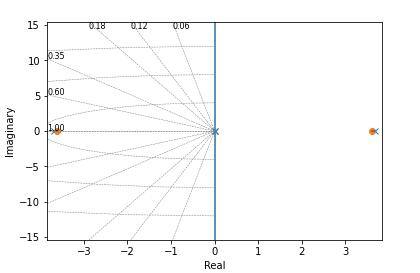
\includegraphics[width=1\linewidth]{images/output/rlocus.jpg}
            \caption{Before pole placement}
            \label{fig:rlocus_before}
        \end{subfigure}
        \begin{subfigure}{.5\textwidth}
          \centering
          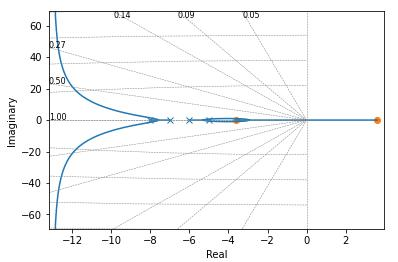
\includegraphics[width=1\linewidth]{images/output/rlocus_tune.jpg}
          \caption{After pole placement}
        \label{fig:rlocus_after}
        \end{subfigure}
    \caption{Root-locus}
    \label{fig:rlocus}
    \end{figure}
        
        At figure \ref{fig:rlocus_before} the root-locus for the initial linearized system is shown, there is a pole at positive half-plane. To stabilize the system, we want all poles to have real parts less than 0, and less poles - faster convergence but with rapid changes.
        
        Let use \textit{scipy.signal.place\_poles} move poles to $[-5, -6, -7, -8]$ in order to balance between fast convergence and rapid acceleration. Changed root-locus (figure \ref{fig:rlocus_after}) shows that system is indeed stable, since there are no asymptotes at positive half plane.
        
        Figures \ref{fig:pole_0}, \ref{fig:pole_1}, \ref{fig:pole_2}, \ref{fig:pole_3}, \ref{fig:pole_4}, \ref{fig:pole_5} show the behaviour of controlled system.

\section*{Task G}
\label{Q:G}
    The LQR controller is shown as python code at \href{https://colab.research.google.com/drive/10-PsTk0fLdFx1oxj48kIPWLQ4z5LQphe}{Google colab}.\\
    Below you can see how the system behave under the LQR controller with different initial conditions $\begin{bmatrix}
            \dot x & \dot\theta & \ddot x & \ddot \theta 
        \end{bmatrix}\T$
    \begin{equation*}
        Q = 100 * \smqty(\imat{4}), R =\smqty(\imat{1})
    \end{equation*}
    For our model it is reasonable to have the following constraint: $-\pi / 2 <= \theta <= \pi / 2 $
    
    From figures \ref{fig:lqr_0}, \ref{fig:lqr_1}, \ref{fig:lqr_2}, \ref{fig:lqr_3}, \ref{fig:lqr_4}, \ref{fig:lqr_5} we can deduce, that state $\bar 0$ is stable, and for other states the LQR with the given $Q$ and $R$ converges in approx. 6 seconds. Also we see at figure \ref{fig:lqr_1} how system behaves if angle in rad is too big which might violate the physics (pendulum shouldn't go through a car) - the graph look pretty reasonable despite very rapid acceleration at the start. Similar rapid acceleration happened at figure \ref{fig:lqr_4}, but this can be tuned by changing $Q$ and $R$ according to the actual problem.
        
        
    \begin{figure}[htb]
        \begin{subfigure}{.5\textwidth}
            \centering
            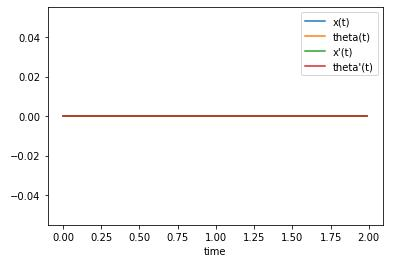
\includegraphics[width=1\linewidth]{images/output/poles/0-0-0-0.jpg}
            \caption{Pole placement}
            \label{fig:pole_0}
        \end{subfigure}
        \begin{subfigure}{.5\textwidth}
          \centering
          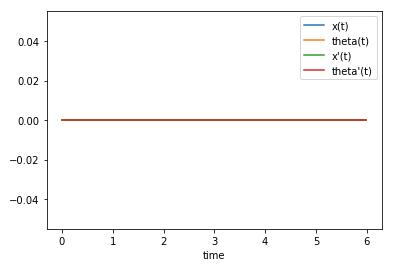
\includegraphics[width=1\linewidth]{images/output/0-0-0-0.jpg}
          \caption{LQR}
        \label{fig:lqr_0}
        \end{subfigure}
    \caption{Stable state [0, 0, 0, 0]}
    \end{figure}
    
    \begin{figure}[htb]
        \begin{subfigure}{.5\textwidth}
            \centering
            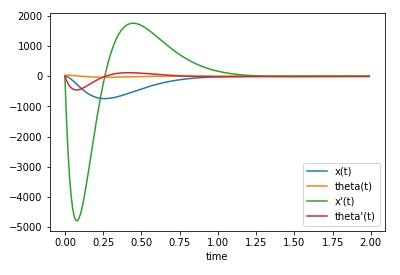
\includegraphics[width=1\linewidth]{images/output/poles/0-40-0-0.jpg}
            \caption{Pole placement}
            \label{fig:pole_1}
        \end{subfigure}
        \begin{subfigure}{.5\textwidth}
          \centering
          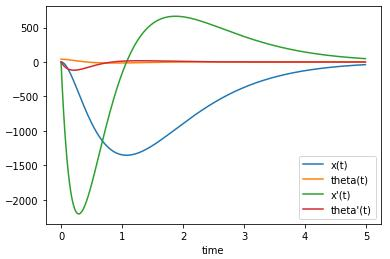
\includegraphics[width=1\linewidth]{images/output/0-40-0-0.jpg}
          \caption{LQR}
        \label{fig:lqr_1}
        \end{subfigure}
    \caption{Big angle: [0, 40, 0, 0]}
    \end{figure}
    
    \begin{figure}[htb]
        \begin{subfigure}{.5\textwidth}
            \centering
            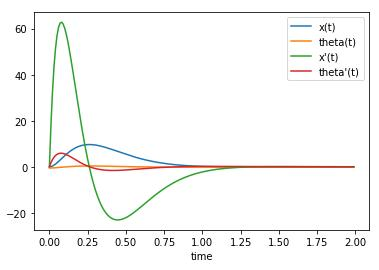
\includegraphics[width=1\linewidth]{images/output/poles/0-neg_pi_6-0-0.jpg}
            \caption{Pole placement}
            \label{fig:pole_2}
        \end{subfigure}
        \begin{subfigure}{.5\textwidth}
          \centering
          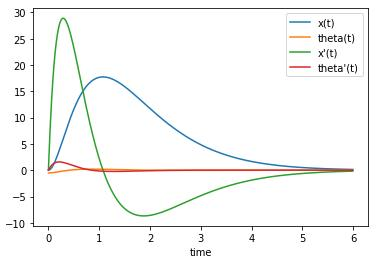
\includegraphics[width=1\linewidth]{images/output/0-neg_pi_6-0-0.jpg}
          \caption{LQR}
        \label{fig:lqr_2}
        \end{subfigure}
    \caption{[0, -$\pi / 6$, 0, 0]}
    \end{figure}
    
    \begin{figure}[htb]
        \begin{subfigure}{.5\textwidth}
            \centering
            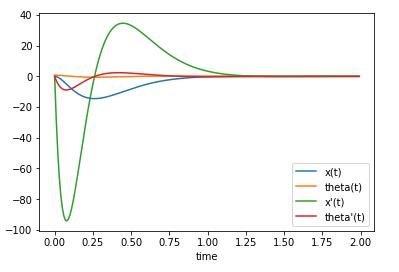
\includegraphics[width=1\linewidth]{images/output/poles/0-pi_4-0-0.jpg}
            \caption{Pole placement}
            \label{fig:pole_3}
        \end{subfigure}
        \begin{subfigure}{.5\textwidth}
          \centering
          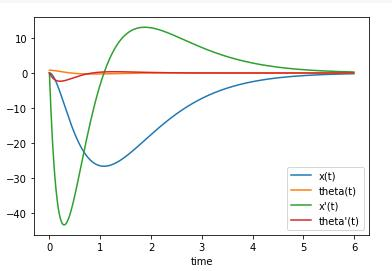
\includegraphics[width=1\linewidth]{images/output/0-pi_4-0-0.jpg}
          \caption{LQR}
        \label{fig:lqr_3}
        \end{subfigure}
    \caption{[0, $\pi / 4$, 0, 0]}
    \end{figure}
        
     \begin{figure}[htb]
        \begin{subfigure}{.5\textwidth}
            \centering
            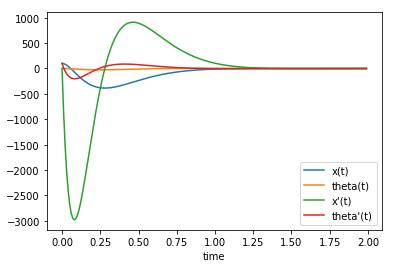
\includegraphics[width=1\linewidth]{images/output/poles/100-0-0-100.jpg}
            \caption{Pole placement}
            \label{fig:pole_4}
        \end{subfigure}
        \begin{subfigure}{.5\textwidth}
          \centering
          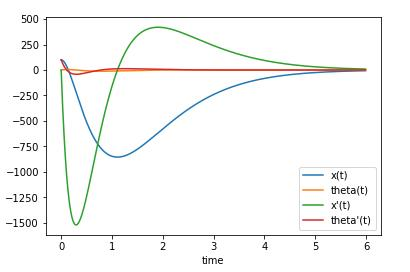
\includegraphics[width=1\linewidth]{images/output/100-0-0-100.jpg}
          \caption{LQR}
        \label{fig:lqr_4}
        \end{subfigure}
    \caption{[100, 0, 0, 100]}
    \end{figure}
    
    \begin{figure}[htb]
        \begin{subfigure}{.5\textwidth}
            \centering
            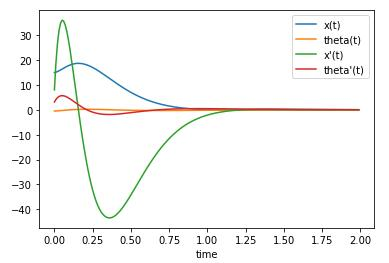
\includegraphics[width=1\linewidth]{images/output/poles/15-neg_pi_6-8-pi.jpg}
            \caption{Pole placement}
            \label{fig:pole_5}
        \end{subfigure}
        \begin{subfigure}{.5\textwidth}
          \centering
          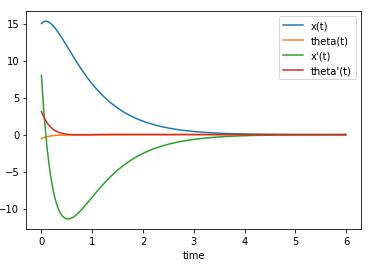
\includegraphics[width=1\linewidth]{images/output/15-neg_pi_6-8-pi.jpg}
          \caption{LQR}
        \label{fig:lqr_5}
        \end{subfigure}
    \caption{[15, $-\pi / 6$, 8, $\pi$]}
    \end{figure}
\end{document}
